\subsubsection{Gravity Acceleration}\label{sssec:gravity-acceleration}

The acceleration of an Earth orbiting satellite due to the Earth's gravity field, 
can be computed using the potential $U$ (see \ref{eq:geopotential})
\begin{equation}
  \bm{\ddot{r}} =  
    \begin{pmatrix} \ddot{x} & \ddot{y} & \ddot{z} \end{pmatrix} = 
    \nabla U
\end{equation}

The classical formulation of the gravitational acceleration derived from the spherical 
harmonics model (see \ref{eq:mont315}) employs the geocentric spherical coordinate 
representation. This formulation results in two singularities at the north and 
south poles (\cite{Atallah2022}). To avoid this problem, our implementation of the 
computation algorithm is based on a development based on Cartesian components, introduced by 
Cunningham (\cite{Cunningham1970}), which is singularity-free. However, this formulation 
is in un-normalized form; an equivalent, normalized form was derived and implemented, 
taking into account \cite{Atallah2022}.

If we define 
\begin{equation}
  \bar{V}_{nm} = \bar{M}_{nm} + i \bar{W}_{nm} = 
    \left( \frac{R_{\Earth}}{r} \right) ^{n+1} \bar{P}_{nm} (\sin \phi) 
      \left( \cos (m\lambda) + i \sin (m\lambda) \right)
\end{equation}

we can rewrite the potential (see \ref{eq:mont310}), as
\begin{equation}
  U = \Re \left( \frac{GM_{\Earth}}{R_{\Earth}} \sum_{n=0}^{\infty} \sum_{m=0}^{n} 
    \left( \bar{C}_{nm} - i \bar{S}_{nm} \right) \bar{V}_{nm} \right)
\end{equation}
using normalized coefficients, so that the acceleration is given by
\begin{equation}
  \bm{\ddot{r}} = \Re \left( \frac{GM_{\Earth}}{R_{\Earth}} \sum_{n=0}^{\infty} \sum_{m=0}^{n} 
    \left( \bar{C}_{nm} - i \bar{S}_{nm} \right) \nabla \bar{V}_{nm} \right)
\end{equation}

Ommiting intermidiate results (see e.g. \cite{Atallah2022}), we end up in the 
recurrence relations:
\begin{equation}
  \begin{aligned}
    \bar{V}_{nm} = B_{nm} \frac{z}{r} \frac{R_{\Earth}}{r} \bar{V}_{n-1,m} 
      - (n+m-1) \frac{B_{nm}}{B_{n-1,m}} \left( \frac{R_{\Earth}}{r} \right) ^2 \bar{V}_{n-2,m} \\
    \bar{M}_{nm} = B_{nm} \frac{zR_{\Earth}}{r^2} \bar{M}_{n-1,m} 
      - \frac{B_{nm}}{B_{n-1,m}} \left( \frac{R_{\Earth}}{r} \right) ^2 \bar{M}_{n-2,m} \\
    \bar{W}_{nm} = B_{nm} \frac{zR_{\Earth}}{r^2} \bar{W}_{n-1,m} 
      - \frac{B_{nm}}{B_{n-1,m}} \left( \frac{R_{\Earth}}{r} \right) ^2 \bar{W}_{n-2,m}
  \end{aligned}
\end{equation}
where 
\begin{equation}
  B_{nm} = \sqrt{\frac{(2n+1)(2n-1)}{(n+m)(n-m)}}
\end{equation}

and for the $n=m$ cases, we have
\begin{equation}
  \begin{aligned}
    \bar{V}_{mm} &= \sqrt{\frac{2m+1}{2m}} \frac{\left(x+iy\right)}{r^2} \bar{V}_{m-1,m-1} \\
    \bar{M}_{mm} &= \sqrt{\frac{2m+1}{2m}} \left( \frac{xR_{\Earth}}{r^2} \bar{M}_{m-1,m-1} 
      - \frac{yR_{\Earth}}{r^2} \bar{W}_{m-1,m-1} \right) \\
    \bar{W}_{mm} &= \sqrt{\frac{2m+1}{2m}} \left( \frac{xR_{\Earth}}{r^2} \bar{W}_{m-1,m-1} 
      + \frac{yR_{\Earth}}{r^2} \bar{M}_{m-1,m-1} \right) \\
  \end{aligned}
\end{equation}

The recurrence starts with initial conditions
\begin{equation}
  \begin{aligned}
    \bar{M}_{00} = \frac{R_{\Earth}}{r} &\text{ and } 
      \bar{M}_{10} = \sqrt{3} \frac{z}{r^2} \bar{M}_{00} \\
    \bar{W}_{00} = 0 &\text{ and } \bar{W}_{10} = 0
  \end{aligned}
\end{equation}

Now we can use the $\bar{M}_{nm}$ and $\bar{W}_{nm}$ to compute the acceleration 
components using
\begin{equation}
  \begin{aligned}
    \ddot{x} & = \sum_{n=0}^{\infty} \sum_{m=0}^{n} \ddot{x}_{nm} \\
    \ddot{y} & = \sum_{n=0}^{\infty} \sum_{m=0}^{n} \ddot{y}_{nm} \\
    \ddot{z} & = \sum_{n=0}^{\infty} \sum_{m=0}^{n} \ddot{z}_{nm}
  \end{aligned}
\end{equation}

where for $m=0$
\begin{equation}
  \begin{aligned}
    \ddot{x}_{n0} &= -\frac{GM_{\Earth}}{R^2_{\Earth}} \frac{N_{n,0}}{N_{n+1,1}}\bar{C}_{n0}\bar{M}_{n+1,1} \\
    \ddot{y}_{n0} &= -\frac{GM_{\Earth}}{R^2_{\Earth}} \frac{N_{n,0}}{N_{n+1,1}}\bar{C}_{n0}\bar{W}_{n+1,1} \\
    \ddot{z}_{n0} &= -\frac{GM_{\Earth}}{R^2_{\Earth}} \frac{N_{n,0}}{N_{n+1,1}} \left(n+1\right) \bar{C}_{n0}\bar{M}_{n+1,0}
  \end{aligned}
\end{equation}

and for $m > 0$
\begin{equation}
  \begin{aligned}
    \ddot{x}_{nm} &= \frac{GM_{\Earth}}{2R^2_{\Earth}} \Bigl( \frac{N_{n,m}}{N_{n+1,m+1}} 
      \left(-\bar{C}_{n,m} \bar{M}_{n+1,m+1} + \bar{S}_{n,m} \bar{W}_{n+1,m+1} \right) \\
       & +\frac{(n-m+2)!}{(n-m)!} \frac{N_{n,m}}{N_{n+1,m-1}}
        \left(-\bar{C}_{n,m} \bar{M}_{n+1,m-1} + \bar{S}_{n,m} \bar{W}_{n+1,m-1} \right) \Bigr) \\
    \ddot{y}_{nm} &= \frac{GM_{\Earth}}{2R^2_{\Earth}} \Bigl( \frac{N_{n,m}}{N_{n+1,m+1}} 
      \left(-\bar{C}_{n,m} \bar{W}_{n+1,m+1} + \bar{S}_{n,m} \bar{M}_{n+1,m+1} \right) \\
       & +\frac{(n-m+2)!}{(n-m)!} \frac{N_{n,m}}{N_{n+1,m-1}}
        \left(-\bar{C}_{n,m} \bar{W}_{n+1,m-1} + \bar{S}_{n,m} \bar{M}_{n+1,m-1} \right) \Bigr) \\
    \ddot{z}_{nm} &= \frac{GM_{\Earth}}{R^2_{\Earth}} \frac{N_{n,m}}{N_{n+1,m}} 
      \left( \left( n-m+1 \right)
      \left(-\bar{C}_{n,m} \bar{W}_{n+1,m+1} + \bar{S}_{n,m} \bar{M}_{n+1,m+1} \right) 
        \right)
  \end{aligned}
\end{equation}

where $N_{nm}$ is the normalization factor for degree $n$ and order $m$
\begin{equation}
  N_{nm} = \sqrt{ \frac{(n-m)! (2n+1) (2-\delta _{0m})}{(n+m)!} }
\end{equation}

\paragraph{Derivative of Acceleration}\label{sssec:derivative-geopotential-acceleration}

Partial derivatives of the acceleration need to be computed, with respect to the 
satellite state vector, $\frac{\partial \bm{\ddot{r}}}{\partial \bm{r}}$ for the variational 
equations. For the central term
\begin{equation}
  \bm{\ddot{r}} = - \frac{GM_{\Earth}}{r^3}\bm{r}
\end{equation}
and using the relation
\begin{equation}
  \frac{\partial r^n}{\partial \bm{r}} = 
    \frac{\partial \left(x^2 + y^2 + z^2 \right)}{\partial \bm{r}} = 
      n \cdot r^{n-2} \cdot \bm{r}^T
\end{equation}
if follows that
\begin{equation}
  \begin{aligned}
    \frac{\partial \bm{\ddot{r}}}{\partial \bm{r}} &= 
    -GM_{\Earth} \frac{\partial}{\partial \bm{r}}\left( \bm{r} \frac{1}{r^3} \right) = 
    -GM_{\Earth} \left( \frac{1}{r^3}\bm{I}_{3\times 3} - 3\bm{r} \frac{\bm{r}^T}{r^5} \right) \\
    &=\frac{-GM_{\Earth}}{{r^5}} \begin{pmatrix}
      3x^2-r^2 & 3xy      & 3xz \\
      3yx      & 3y^2-r^2 & 3yz \\
      3zx      & 3zy      & 3z^2 -r^2
    \end{pmatrix}
  \end{aligned}
\end{equation}
which shows that the gravity gradient is symmetric and with a zero trace. The same result 
can be deduced considering earth's gravitational potential expressed as \ref{eq:mont34} 
(see \cite{Montenbruck2000}). The two properties reduce the number of independent 
components that have to be considered in the computation from nine to five. 

Deriving the partials is quite tedius. For the computation, we follow the development 
used in \ref{sssec:gravity-acceleration}, follwing a normalized version of 
\cite{Cunningham1970} to compute the quantities $\frac{\partial \ddot{x}_{nm}}{\partial x}$, 
$\frac{\partial \ddot{x}_{nm}}{\partial y}$, $\frac{\partial \ddot{x}_{nm}}{\partial z}$, 
$\frac{\partial \ddot{y}_{nm}}{\partial z}$ and $\frac{\partial \ddot{z}_{nm}}{\partial z}$.

\paragraph{Earth Rotation}\label{sssec:gravity-acceleration-earth-rotation}

Formulas presented in the current section, \ref{sssec:gravity-acceleration}, 
are valid in an \gls{ecef} frame, that is ignore Earth's rotation (aka $\bm{r}$ is 
the satellite's position vector in \gls{ecef} coordinates). We are now designating 
the $\bm{r}$ vector as $\bm{r}_{ef}$ and introducing $\bm{r}_{sf}$ to designate the 
correspongind celestial, ``space-fixed'' vector, with 
\begin{equation}
  \bm{r}_{ef} = \bm{R} \cdot \bm{r}_{sf}
\end{equation}
where $\bm{R}$ is the terretrial-to-celestial transformation matrix. The partial 
derivatives $\frac{\partial \bm{\ddot{r}}}{\partial \bm{r}}$ is the ``space-fixed'' 
frame, would then be given by
\begin{equation}
  \left( \frac{\partial \bm{\ddot{r}}}{\partial \bm{r}} \right) _{sf} = 
  \bm{R}^T 
  \left( \frac{\partial \bm{\ddot{r}}}{\partial \bm{r}} \right) _{ef}
  \bm{R}
\end{equation}
and for the acceleration
\begin{equation}
  \bm{\ddot{r}}_{sf} = \bm{R}^T \cdot \bm{\ddot{r}}_{ef}
\end{equation}

\paragraph{Validation}\label{sssec:gravity-acceleration-acceleration}

The acceleration induced to an earth orbiting satellite by the earth's gravity 
field, is by far the largest in magnitude, hence it should be computed with utmost 
precision. To test our implementation, we checked our results against the \texttt{COST-G} 
benchmark test. Input data for the test is a one day orbit arc of \gls{grace} paired
with the earth gravity model \texttt{EIGEN-6C4}. Acceleration is evaluated from degree
and order 2 to 180 (i.e. leaving out the largest in magnitude central term). According 
to \cite{Lasser23}, accelerations should be consistent to at least \SI{10e-12}{\metre\per\square\second}.
The discrepancies between our implementation and the benchmark test are depicted in 
\ref{fig:costg-benchmark-02gravityfield-itrf} and \ref{table:costg-benchmark-02gravityfield-itrf}. 
It is clear that results obtained lie within the accuracy demands of the benchmark test.

\begin{figure}
  \centering
  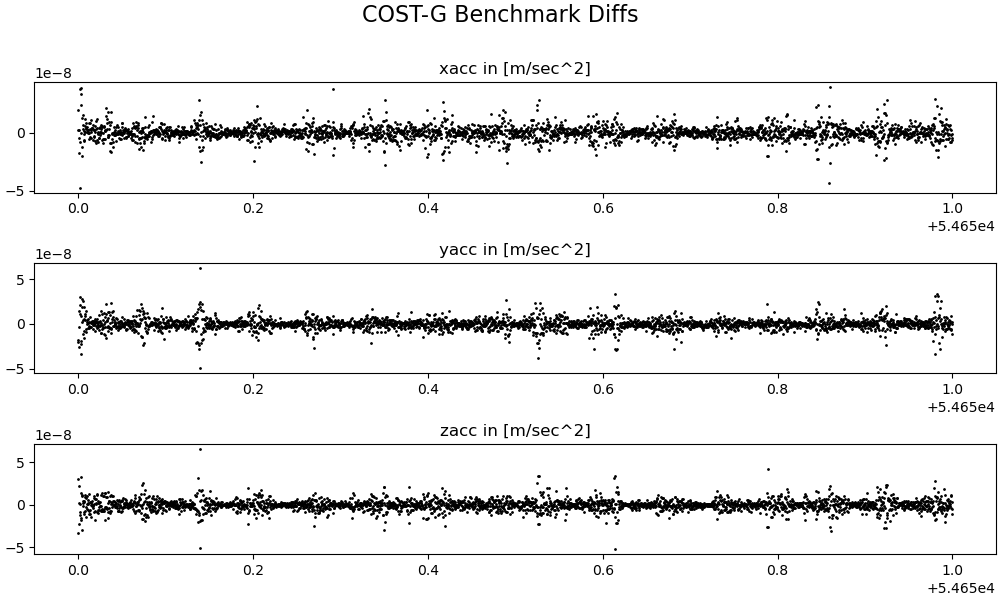
\includegraphics[height=.4\textheight,keepaspectratio]{02gravityfield_itrf}
  \caption{Earth gravity acceleration descripancies against the \texttt{COST-G} 
    benchmark test. Gravity model is \texttt{EIGEN-6C4} from degree and order 2 to 180. 
    Comparing results for a one day orbit arc of \gls{grace} in \gls{itrf}.}
  \label{fig:costg-benchmark-02gravityfield-itrf}
\end{figure}

\begin{table}[h!]
  \centering
  \begin{tabular}{ccccc}
      %\hline
      \textbf{Component} & \textbf{Min} & \textbf{Max} & \textbf{Mean} & \textbf{Std. Deviation}\\
      & \multicolumn{4}{c}{\si{\metre\per\square\second}} \\
      \hline
      $\ddot{x}$ & -1.28e-15 & +1.79e-15 & -1.00e-18 & 2.64e-16 \\
      $\ddot{y}$ & -1.52e-15 & +1.32e-15 & -3.43e-18 & 2.58e-16 \\
      $\ddot{z}$ & -1.14e-15 & +1.00e-15 & -5.81e-18 & 2.19e-16 \\
      \hline
  \end{tabular}
  \caption{Earth gravity acceleration descripancies against the \texttt{COST-G} benchmark test.}
  \label{table:costg-benchmark-02gravityfield-itrf}
\end{table}
